\documentclass[12pt,a4paper]{article}

\usepackage[T1]{fontenc}
\usepackage{mathptmx}
\usepackage{setspace}
\usepackage{graphicx}
\usepackage{lipsum}
\usepackage{atbegshi}
\usepackage{geometry}
\usepackage{layout}
\usepackage{enumitem}
\usepackage{listings}
\usepackage[skip=5pt plus1pt, indent=20pt]{parskip}

\lstdefinelanguage
   [x64]{Assembler}     % add a "x64" dialect of Assembler
   [x86masm]{Assembler} % based on the "x86masm" dialect
   % with these extra keywords:
   {morekeywords={CDQE,CQO,CMPSQ,CMPXCHG16B,JRCXZ,LODSQ,MOVSXD, %
                  POPFQ,PUSHFQ,SCASQ,STOSQ,IRETQ,RDTSCP,SWAPGS, %
                  rax,rdx,rcx,rbx,rsi,rdi,rsp,rbp, %
                  r8,r8d,r8w,r8b,r9,r9d,r9w,r9b, %
                  r10,r10d,r10w,r10b,r11,r11d,r11w,r11b, %
                  r12,r12d,r12w,r12b,r13,r13d,r13w,r13b, %
                  r14,r14d,r14w,r14b,r15,r15d,r15w,r15b}} % etc.

\lstset{language=[x64]Assembler}


\graphicspath { {./img/} }
% \geometry{lmargin=4.0cm, tmargin=4.0cm, rmargin=3.0cm, bmargin=3.0cm}
\setstretch{1.5}
\renewcommand{\baselinestretch}{1.0}
\renewcommand{\figurename}{Gambar.}
\date{}

\title{

  {\Huge{Arsitektur dan Organisasi Komputer: CPU}}

  {\large{MAKALAH}}

  {\normalsize{DISUSUN OLEH}}

  {\Large{Radinal Shidiq Saragih}}

  {\normalsize{5520123104}}

  {\vspace{1cm}}
  {
\includegraphics[scale=0.2]{cover/logo_unsur.png}}
  {\vspace{1cm}}

  {\large{PROGRAM STUDI TEKNIK INFORMATIKA}}

  {\large{FAKULTAS TEKNIK}}

  {\large{UNIVERSITAS SURYAKANCANA}}

  {\large{CIANJUR}}

  {\small{2024}}
}


\begin{document}

  \pagenumbering{gobble}

  \begin{titlepage}
    \maketitle
  \end{titlepage}

  \newpage

  \pagenumbering{roman}
  \setcounter{page}{1}

  \begin{center}
    \Large{\textbf{KATA PENGANTAR}}
  \end{center}

  \vspace{0.5cm}

  Puji dan syukur penyusun panjatkan kepada Tuhan Yang Maha Esa atas berkat dan
rahmat-Nyalah sehingga penyusun dapat menyelesaikan makalah yang berjudul Arsitektur
dan Organisasi Komputer: CPU.

Adapun tujuan dari pembuatan makalah ini adalah untuk memenuhi tugas mata kuliah
Arsitektur dan Organisasi Komputer.

Tak lupa penyusun juga mengucapkan terimakasih yang sebanyak-banyaknya kepada
setiap pihak yang telah mendukung serta membantu penyusun selama proses penyelesaian
tugas ini. Ucapan terima kasih penyusun sampaikan kepada.

\begin{itemize}
  \item{Ibu Siti Nazilah. selaku dosen mata kuliah}
  \item{Teman-teman Kelompok 3} \dots{}
    \begin{itemize}
        \item Devina Fauzia Sari Efendi (5520123082)
        \item Ajeng Salma Syafiatun Najaa (5520123078)
        \item Aliman Sayful Aziz (5520123079)
        \item Arief Moch Yusup (5520123080)
    \end{itemize}
\end{itemize}

Pada makalah ini akan dibahas tentang \textit{Central Processing Unit} (\textit{CPU})
atau disebut juga dengan prosesor, komponen-komponen yang terdapat didalamnya,
dan bagaimana komponen tersebut berkerja sama dalam suatu organisasi arsitektur CPU.

Meskipun telah berusaha menyelesaikan makalah ini dengan sebaik mungkin,
penyusun menyadari bahwa makalah ini masih ada kekurangan. Oleh karena itu,
penyusun mengharapkan kritik dan saran yang membangun dari semua pihak,
guna menyempurnakan segala kekurangan dalam makalah ini.

\vspace{1cm}

\begin{center}
  \begin{flushright}
    Cianjur, 16 Februari 2024

    Penyusun
  \end{flushright}
\end{center}


  \addcontentsline{toc}{section}{KATA PENGANTAR}{}

  \newpage


  \newpage

  \renewcommand\contentsname {\Large{\textbf{DAFTAR ISI}} }

  \setcounter{page}{2}
  % \addcontentsline{toc}{section}{DAFTAR ISI}{}

  \begin{center}
  \tableofcontents
  \end{center}

  \newpage

  \pagenumbering{arabic}
  \setcounter{page}{1}

  \begin{center}
    \Large{\textbf{PENDAHULUAN}}
  \end{center}

  \vspace{0.5cm}

  \section*{BAB I: PENDAHULUAN}
  \addcontentsline{toc}{section}{BAB I: PENDAHULUAN}{}
  \setcounter{section}{1}
  \setcounter{subsection}{0}
  \subsection{Latar Belakang}

Dalam era perkembangan teknologi informasi yang pesat, pemahaman terhadap
Central Processing Unit (CPU) menjadi sangat krusial. CPU, atau sering
disebut prosesor, merupakan otak dari setiap sistem komputer. Sebagai komponen inti,
CPU bertanggung jawab untuk menjalankan instruksi-instruksi yang diberikan
oleh perangkat lunak dan mengendalikan operasi-operasi dasar pada tingkat tinggi.

Kemampuan dan kinerja CPU memiliki dampak langsung terhadap kecepatan dan
efisiensi suatu sistem komputer. Oleh karena itu, pemahaman yang mendalam
terhadap arsitektur dan organisasi CPU sangat penting, terutama bagi mahasiswa
yang mengambil mata kuliah Arsitektur dan Organisasi Komputer.

Dengan adanya pemahaman yang mendalam terhadap CPU, diharapkan pembaca
dapat mengaplikasikan pengetahuan ini dalam konteks yang lebih luas,
seperti pengembangan perangkat lunak, perancangan sistem, dan pemecahan
masalah dalam dunia teknologi informasi. Melalui eksplorasi terhadap CPU,
diharapkan pula bahwa mahasiswa dapat membangun dasar yang kuat untuk pemahaman
lebih lanjut dalam bidang komputer dan teknologi informasi.

\subsection{Tujuan Masalah}

\begin{enumerate}[label=\alph*.]
  \item Terdiri dari apa sajakah suatu CPU?
  \item bagaimana bagian-bagian suatu CPU berinteraksi dan bekerja sama?
  \item Apa yang dimaksud dengan operasi mikro?
  \item Apa saja jenis operasi mikro?
\end{enumerate}


  \newpage

  \section*{BAB II: PEMBAHASAN}
  \addcontentsline{toc}{section}{BAB II: PEMBAHASAN}
  \setcounter{section}{2}
  \setcounter{subsection}{0}

    \subsection{Pengertian CPU}
    Central Processing Unit atau CPU adalah komponen elektronik yang didalam suatu sistem komputer bertugas
untuk mengendalikan dan mengatur keseluruhan sistem, mulai dari perhitungan-perhitungan,
alokasi memori hingga kendali atas I/O sistem.

\begin{flushleft}
Berikut adalah beberapa definisi dari CPU menurut para ahli.
\end{flushleft}

\begin{enumerate}[label=\alph*.]
  \item Tanenbaum dan Austin (2012): Definisi dari dari CPU menurut Tanenbaum dan Austin adalah``\textit{CPU} (\textit{Central Processing Unit}) adalah otak dari sebuah komputer. Yang berfungsi untuk menerima instruksi, memprosesnya, dan menjalankannya satu per satu``.
  \item Wilson (2018): Menurut Wilson, ``CPU atau prosessor adalah otak dari sebuah komputer dan akan merespon perintah yang diberikan oleh user. CPU juga adalah salah satu faktor penting dalam menentukan kekuatan sebuah sistem``.
  \item Institute of Electrical and Electronics Engineers (IEEE) : menurut IEEE di dalam Standard Glossary of Computer Hardware Terminology (1999), CPU adalah ``Sebuah alat yang mengartikan dan menjalankan instruksi, terdiri dari Control Unit Instruksi dan Unit Aritmatika``.
\end{enumerate}


    \subsection{Peran dan Fungsi CPU}
    CPU adalah bagian dimana segala pemrosesan data dilaksanakan.
Dan sebagai ``otak`` dari suatu sistem terdapat banyak pekerjaan yang dikerjakan oleh CPU, antara lain.

\begin{enumerate}[label=\alph*.]
  \item Eksekusi Instruksi
  \item Operasi Aritmatika dan Logika (ALU)
  \item Pengelolaan Register
  \item Pengaturan Bus Sistem
  \item Pemrosesan Input/Output (I/O)
  \item Manajemen Interrupt
  \item Manajemen Kesalahan:
  \item Pemrosesan Paralel (Multi-Core)
  \item Manajemen Kinerja dan Daya
\end{enumerate}

Peranan penting dan fungsionalitas yang dipegang oleh sebuah CPU merupakan komponen yang menentukan
keberhasilan atau kegagalan suatu sistem komputer dalam menjalankan tugasnya.


    \subsection{Prinsip Dasar Kerja CPU}
      \begin{figure}[h]
    \centering
    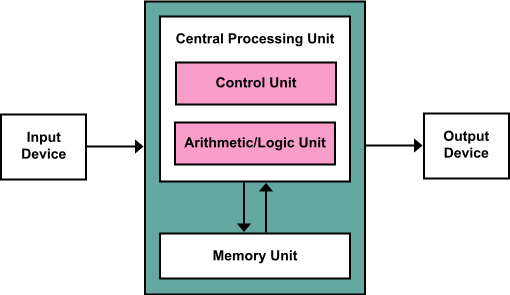
\includegraphics[scale=0.5]{CPUBASICDIAG}
    \caption{Diagram Sederhana CPU}
    \label{fig:CPUBASICDIAG}
\end{figure}

Cara kerja suatu CPU dapat digambarkan secara sederhana sepeti di Gambar\ref{fig:CPUBASICDIAG}.
Di diagram tersebut dapat dilihat ada tiga Unit Dasar CPU yang bertugas untuk melakukan
kalkulasi-kalkulasi penting bagi komputer.

Secara tingkatan, sebuah Control Unit adalah Unit terpenting, karena ialah yang mengatur
unit-unit lain yang dibawahnya, kemudian diikuti oleh Unit Arithmetic-Logic yang
adalah bagian dimana semua perhitungan aritmatika dan logika terjadi, dan terakhir
adalah Memory Unit, yang mempercepat kerja kedua unit yang lain tersebut, karena
di unit ini CPU bisa dapat media penyimpanan yang berkecepatan tinggi.

Suatu CPU ketika berkerja, akan menerima instruksi dari program-program yang menyala
di komputer, dan kemudian memproses instruksi tersebut menggunakan ketiga unit yang
telah disebut itu dan kemudian akan meng-outputkan nilai atau hasil sesuai dengan
instruksi.


    \subsection{Bagian-Bagian CPU}
      Dengan berjalannya waktu, telah dikembangkan jutaan bahkan ratusan juta
rancangan CPU yang berbeda-beda, namun sebuah CPU pada dasarnya akan memiliki
hal-hal sebagai berikut.

\begin{enumerate}
  \item Unit Control
  \item Unit Aritmatika (ALU)
  \item Unit Memori
\end{enumerate}


      \subsubsection{Unit Control}
        Unit Control CPU adalah bagian dari CPU yang sangat penting dalam memastikan CPU
berjalan sebagaimana seharusnya.

Dalam suatu organisasi suatu CPU, unit control tersebut mengatur tugas antara
bagian CPU, agar instruksi yang didapatkan CPU dapat dijalankan secara sistematis.

Unit ini terdiri atas beberapa sub-unit atau elemen yang masing-masing memiliki
fungsi dan tugas tersendiri.

Menurut Prasetyo B., Puspitasari, A., dan Nasution, R, (2019), Unit Control adalah ``Elemen Control unit merujuk pada bagian dari sebuah sistem komputer yang bertanggung jawab
untuk mengarahkan dan mengkoordinasikan aktivitas seluruh unit fungsional dalam pemrosesan data``.

Berikut adalah unit internal yang umumnya terdapat dalam Unit Control CPU.

\begin{enumerate}[label=\alph*.]

  \item \textbf{ Control Lines}

    Sinyal-sinyal yang mengatur operasi dalam suatu unit pemrosesana, contohnya
    proses \textit{read/write} atau untuk mengirim sinyal agar mengaktifkan ALU
    (Arithmetic Logic Unit).

  \item \textbf{ ALU Control Unit}

    Bagian yang mengontrol operasi-operasi aritmatika yang dilakukan ALU
    (penambahan, pengurangan, perkalian, atau operasi logika).


  \item \textbf{ Clock Circuit }

    Bagian yang mengatur alur waktu dalam pengeksekusian instruksi, agar
    dieksekusi dengan urutan yang tepat.

  \item \textbf{ Bus Interface Unit }

    Bagian yang berada diantara CPU dengan sistem bus komputer, dan bagian inilah
    yang memberikan CPU akses ke komputer secara keseluruhan, seperti RAM, ataupun
    perangkat I/O.

  \item \textbf{ Control Unit Sequencer }

    Bagian yang memastikan langkah-langkah instruksi memiliki urutan yang benar
    agar dapat dieksekusi dengan tepat (Sequencing Logic).

  \item \textbf{ Decoder }

    Decoder atau Unit Decoder, adalah bagian Control Unit yang berfungsi
    untuk memproses instuksi tersebut dan menghasilkan sinyal-sinyal kontrol
    yang sesuai.

\end{enumerate}


      \subsubsection{Unit Pemrosesan Aritmatika dan Logika (ALU)}
        \begin{figure}[h]
    \centering
    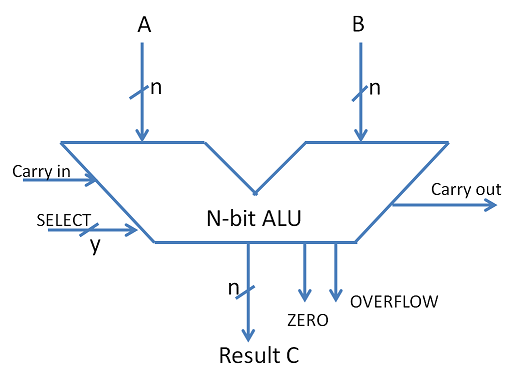
\includegraphics[scale=0.5]{ALUSYMBOLDIAG}
    \caption{Diagram Unit ALU}
    \label{fig:ALUSYMBOLDIAG}
\end{figure}

Arithmetic Logic Unit atau ALU adalah unit atau bagian CPU yang bertugas untuk
memproses kalkulasi-kalkulasi aritmatika dan operasi boolean/logika.

Menurut Ensiklopedia Brittanica, Arithmetic Logic Unit (ALU) adalah ``\dots{}unit yang
berkaitan dengan empat fungsi aritmatika dasar, yaitu pertambahan, pengurangan,
perkalian, dan pembagian, serta operasi logika tertentu seperti perbandingan antara data
dan dalam memilih prosedur untuk menjawab suatu masalah atau bedasarkan kriteria yang
sudah ditentukan diawal.\dots{}``

Secara struktural unit ini terdiri dari gerbang-gerbang logika semikonduktor
yang kemudian disusun hingga dapat memproses nilai-nilai integer biner.

Dan karena ALU hanya memproses nilai integer, terdapat juga unit yang memproses nilai-nilai
floating-point atau decimal. Unit ini disebut dengan Floating-Point Unit atau FPU.

FPU berbeda dari ALU karena, dengan ALU yang umumnya ditemui di chipset suatu CPU,
FPU lebih sering ditemui diluar chipset, dan terletak di suatu tempat lain di Motherboard.

Di diagram Gambar~\ref{fig:ALUSYMBOLDIAG} dapat disimpulkan beberapa hal, pertama suatu ALU
akan menerima dua input (A dan B di diagram), ALU juga menerima sinyal operasi apa yang akan
digunakan (SELECT di diagram), akan mengeluarkan status yang dikirim ke register yang menyimpan
status akhir suatu operasi(Carry in, Carry out, Overflow dan Zero), dan terakhir akan mengoutput
nilai dari kedua data yang telah dioperasikan.

Dan selain FPU, terdapat juga yang bernama GPU yang bertugas untuk memproses instruksi-instruksi
grafis, GPU sendiri adalah Evolusi dari cara komputer-komputer lama yang hanya bergantung
kepada CPU untuk memproses grafis. Dalam hal lokasi dimana GPU ini terletak terdapat dua variasi
yaitu GPU yang terpisah dari GPU entah itu terletak di suatu chip di motherboard atau sebagai
peripheral PCIe, dan ada juga yang terletak didalam chipset atau APU atau dengan kata lain
Integrated GPU.


      \subsubsection{Unit Memori}
        Di dalam suatu komputer sudah pasti ada suatu mekanisme penyimpanan, contohnya
seperti memori utama yang dimiliki sistem seperti RAM (Random Access Memori).

\begin{figure}[h]
    \centering
    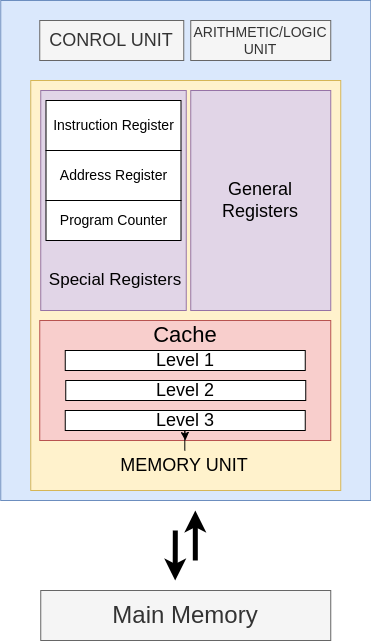
\includegraphics[scale=0.5]{MEMUNITDIAG}
    \caption{Diagram Unit Memori}
    \label{fig:MEMUNITDIAG}
\end{figure}

Namun selain RAM, CPU pun memiliki tempat penyimpanan tersendiri yang kecil didalam
chipset CPU itu sendiri, media penyimpanan tersebut disebut dengan Memori Unit.

Didalam suatu CPU, terdapat dua jenis Memori Unit yang kerap dijumpai,
yaitu Register dan juga System Cache atau CPU Cache.

Perbedaan antara Register dengan Sistem Cache terletak pada ukuran memori yang
dimiliki serta kegunaan yang mereka miliki. Berikut adalah penjelasannya.

\begin{enumerate}
  \item \textbf{Register}

    Register adalah tempat-tempat penyimpanan yang relatif berukuran kecil,
    yang terletak di dalam chipset suatu CPU.

    Karena register terletak sangat dekat dengan cpu, kecepatan dalam hal-hal
    seperti untuk read-write ke dalam memori tersebut dapat dilakukan dengan
    sangat cepat.

    Tidak ada batasan dalam berapa register yang dapat dimiliki suatu register,
    dan register dapat dibagi kedalam dua tipe bedasarkan fungsi, yaitu
    Special Register (Register Khusus), atau General Register.

    Special Register adalah register-register yang memiliki fungsi khusus yang
    sudah ditetapkan oleh rancangan suatu CPU, maka register-register ini
    berkaitan erat dengan proses-proses yang berlangsung didalam suatu CPU.

    Selain Special Register, terdapat juga General Register atau General Purpose
    Register, General Purpose Register ini adalah register-register yang tidak
    memiliki fungsi khusus dan dapat digunakan secara bebas karena tidak terikat
    dengan proses CPU.

    Special Register memiliki beberapa tipe bedasarkan fungsi atau data yang
    ia simpan, berikut adalah tipe-tipenya.

    \begin{itemize}

      \item \textbf{Current Instruction Register (CIR/IR)}

        Register yang menyimpan alamat memori dari instruksi yang
        sedang diproses.

      \item \textbf{ Program Counter Register  (PC) }

        Register yang menyimpan alamat memori selanjutnya dari suatu instruksi
        yang akan dijalankan.

      \item \textbf{Accumulator (AC)}

        Register yang menyimpan informasi terakhir dari suatu data yang diakses
        dari memori.

      \item \textbf{Memory Address Register (MAR)}

        Register yang menyimpan alamat memori yang dapat diakses jika diperlukan.

      \item \textbf{Memory Data Register (MDR) dan Memory Buffer Register (MBR)}

        Register yang menyimpan data yang akan di akses atau dikirim ke memori.

      \item \textbf{Condition Code Register}

        Register yang menyimpan status akhir dari suatu operasi.

      \item \textbf{Temporary Register}

        Register yang hanya menyimpan data-data sementara.

      \item \textbf{Input Register}

        Register yang menyimpan sebuah karakter dari input.

      \item \textbf{Input Register}

        Register yang menyimpan sebuah karakter dari ouput.

      \item \textbf{Index Register (BX)}

        Register ini menyimpan nilai dari suatu alamat memori dan merubahnya
        menjadi alamat efektif untuk digunakan dalam merubah suatu alamat dari
        data yang di operasikan.

      \item \textbf{Stack Control Registers (SCR)}

        Suatu set memori register yang berbentuk tumpukan atau \textit{stack},
        yang dalam mengakses menggunakan metode LIFO atau Last in First Out, yang
        artinya data yang pertama kali di tambahkan atau berada di tumpukan paling
        bawah hanya bisa diakses setelah telah mengakses terlebih dahulu data
        yang berada diatasnya.

      \item \textbf{Flag Register (FR)}

        Suatu set Register yang menyimpan suatu keadaan (\textit{Flag}) suatu kondisi,
        biasanya berukuran 8 bytes dengan tiap kondisi digambarkan dengan data
        atau susunan bit berukuran 8 bit.

        Ada beberapa jenis keadaan yang disimpan, yaitu.

        - \textit{Zero flags}

        - \textit{Carry flag}

        - \textit{Parity flag}

        - \textit{Sign flag}

        - \textit{Overflow flag}

      \item \textbf{Segment Register (SR)}

        Menyimpan alamat suatu memori

      \item \textbf{Data Register (DX)}

        Menyimpan alamat suatu memori suatu data yang akan dioperasikan

    \end{itemize}

    Ukuran atau besar penyimpanan sebuah register sangat beragam, tergantung
    rancangan suatu CPU, misalkan di arsitektur moderen seperti X86\_64 ukuran
    yang dimiliki suatu register berada diantara 8 bit hingga 64 bit.

    Dan batasan yang dimiliki register pun adalah salah satu penyebab suatu
    program komputer yang ditulis untuk CPU 64 bit keatas tidak bisa langsung
    dijalankan di CPU yang ber-arsitektur 32 bit tanpa dibuat suatu lapisan
    translasi yang merubah instruksi 64 bit ke dalam 32 bit.

    Register di tiap-tiap arsitektur CPU memiliki nama-nama khusus yang berguna
    untuk mengindentifikasi satu sama lainnya. Misalkan di arsitektur x86\_64
    RAX adalah label untuk sebuah General Register yang berukuran 64bit, atau
    RFLAGS yang merupakan label untuk suatu Status Register (mirip dengan Condition Register).

  \item \textbf{System Cache}

    System Cache atau CPU Cache adalah lapisan caching yang mempercepat proses
    pembacaan data dari memori utama (RAM).

    Bedasarkan Ensiklopedia Britannica, Cache atau Cache Memory adalah
    ``Memori tambahan yang secara sementara menyimpan instruksi dan data yang
    sering diakses agar dapat diproses lebih cepat oleh Central Processing Unit
    (CPU)``.

    Dalam CPU, terdapat beberapa tingkatan atau level cache, sebagaimananya dapat
    dilihat di Gambar \ref{fig:MEMUNITDIAG}. Untuk kecepatan, semakin lapisan cache
    terletak lebih dekat dengan CPU ia akan memiliki kecepatan yang lebih cepat.

    Di Gambar \ref{fig:MEMUNITDIAG}, terdapat tiga tingkatan cache sebelum
    bertemu langsung dengan RAM. Dalam mengakses data, CPU akan mulai dari lapisan tercepat,
    yaitu L1 cache atau Level 1 cache di Diagram tersebut dan ia akan mencari terus
    dari cache level 1 tersebut hingga level terakhir (L3 di diagram), dan jika data yang
    dicari belum ditemukan CPU lalu akan mencari langsung ke RAM.

    Struktur caching ini adalah penyebab kenapa sekelompok data di memory yang
    memiliki elemennya terpisah-pisah diantara suatu bongkahan memori akan lebih lambat
    untuk diakses dibanding suatu struktur data yang tersusun secara berurutan. Contoh
    dari ini adalah perbandingan antara struktur data Array dibandingkan Linked List.

\end{enumerate}


    \subsection{Pengertian Operasi Mikro}
        Operasi Mikro atau Micro-operations (Micro-Ops) adalah operasi tingkat rendah
yang berfungsi untuk mengimplementasi perintah-perintah bahasa mesin.

Operasi ini biasanya melakukan sejumlah operasi-operasi terhadap data di satu
atau lebih register.

Ketika sebuah program komputer berjalan, akan terdapat sejumlah siklus instruksi yang akan
disampaikan kepada CPU, dan instruksi tersebut direpresentasikan dengan opcode atau Operation-Code.

Opcode akan disampaikan ke Control Unit CPU untuk diproses dan diartikan oleh Unit Decoder, yang
akan menghasilkan sekelompok instruksi-instruksi yang sederhana yang akan di salurkan ke
control lines yang sesuai dengan jenis instruksi. Operasi ini disebut dengan Operasi Mikro.


    \subsection{Jenis-Jenis Operasi Mikro}
        Terdapat beberapa jenis operasi mikro, antara lain.

\begin{enumerate}[label=\alph*]

  \item \textbf{Operasi Aritmatika}
    \begin{enumerate}[label=\roman*.]
      \item Penambahan (ADD): Melibatkan penjumlahan dua operand.
      \item Pengurangan (SUB): Melibatkan pengurangan satu operand dari operand lain.
      \item Perkalian (MUL): Melibatkan perkalian dua nilai atau register.
      \item Pembagian (DIV): Melibatkan pembagian satu nilai oleh yang lain.
    \end{enumerate}

  \item \textbf{Operasi Bitwise Logika}
    \begin{enumerate}[label=\roman*.]
      \item AND Logika (AND): Melibatkan operasi AND bit-wise antara dua operand.
      \item OR Logika (OR): Melibatkan operasi OR bit-wise antara dua operand.
      \item XOR Logika (XOR): Melibatkan operasi XOR bit-wise antara dua operand.
      \item NOT Logika (NOT): Melibatkan operasi NOT bit-wise pada suatu operand.
    \end{enumerate}

  \item \textbf{Operasi Pergeseran Bit (Bitshift)}
    \begin{enumerate}[label=\roman*.]
      \item Pergeseran Kiri (Shift Left): Menggeser bit-bit suatu operand ke kiri.
      \item Pergeseran Kanan (Shift Right): Menggeser bit-bit suatu operand ke kanan.
    \end{enumerate}

  \item \textbf{Operasi Perbandingan}
    \begin{enumerate}[label=\roman*.]
      \item Operasi Setara (Equal): Membandingkan apakah dua operand setara.
      \item Operasi Kurang dari (Less Than): Membandingkan apakah satu operand kurang dari operand lain.
    \end{enumerate}

  \item \textbf{Operasi Load/Store}
    \begin{enumerate}[label=\roman*.]
      \item Load (Memuat): Memuat nilai dari suatu lokasi memori ke dalam register.
      \item Store (Menyimpan): Menyimpan nilai dari register ke dalam lokasi memori.
    \end{enumerate}

  \item \textbf{Operasi Kontrol Aliran}
  \begin{enumerate}[label=\roman*.]
    \item Operasi Skala (Jump): Melibatkan lompatan ke alamat tertentu berdasarkan kondisi tertentu.
    \item Operasi Panggil (Call): Melibatkan pemanggilan suatu subrutin atau fungsi.
  \end{enumerate}

  \item \textbf{Operasi Pemindahan Data}
  \begin{enumerate}[label=\roman*.]
    \item Pindah Register ke Register: Memindahkan nilai dari satu register ke register lain.
    \item Pindah Memori ke Register: Memuat nilai dari lokasi memori ke dalam register.
  \end{enumerate}

\item \textbf{Operasi Kontrol Aliran}
    \begin{enumerate}[label=\roman*.]
      \item Membaca Memori (Memory Read): Membaca nilai dari lokasi memori.
      \item Menulis ke Memori (Memory Write): Menulis nilai ke dalam lokasi memori.
    \end{enumerate}

  \item \textbf{Operasi Pemrosesan Floating-Point}
    \begin{enumerate}[label=\roman*.]
      \item  Operasi Aritmatika Floating-Point: Melibatkan operasi aritmatika untuk nilai floating-point.
    \end{enumerate}

  \item \textbf{Operasi Pemrosesan String}
  \begin{enumerate}[label=\roman*.]
    \item Manipulasi String: Melibatkan operasi penggabungan dan pemisahan karakter dalam string.
  \end{enumerate}

  \item \textbf{Operasi Kontrol Sirkuit Internal}
  \begin{enumerate}[label=\roman*.]
    \item  Pengaturan dan Kontrol Sirkuit Internal CPU: Mengendalikan berbagai elemen dan sirkuit internal di dalam CPU.
  \end{enumerate}

\end{enumerate}


  \newpage

  \section*{BAB III: PENUTUP}
  \addcontentsline{toc}{section}{BAB III: PENUTUP}
  \setcounter{section}{3}
  \setcounter{subsection}{0}
  \subsection{Kesimpulan}

Kesimpulan yang didapat adalah, dalam CPU atau Central Processing Unit terdapat
tiga unit terpenting yaitu,

\begin{itemize}
  \item Control unit
  \item Arithmetic/Logic Unit (ALU)
  \item Memory Unit
\end{itemize}

Dengan control unit bertugas untuk mengatur dua unit lainnya, Arithmetic/Logic Unit
atau ALU bertugas untuk melakukan perhitungan-perhitungan yang diperlukan dan proses
ini dibantu dengan Memory Unit yang terdiri dari cache dan register, fungsi utama dari
unit ini adalah untuk menyediakan tempat penyimpanan untuk data-data yang sedang di proses CPU.

Dan di tingkat mikro, terdapat istilah operasi mikro yang mengacu kepada operasi tingkat
bit yang dilakukan oleh gerbang-gerbang logika yang berada di control unit CPU. Operasi Mikro
berasal hasil representasi instruksi yang disampaikan kepada CPU ketika sebuah program berjalan
representasi ini berbentuk biner dan disebut dengan opcode atau Operation-Code.

\subsection{Saran}

Agar lebih memahami operasi yang berada di tingkat CPU, perlu juga dipelajari
pemograman di tingkat rendah yang berbentuk assembly. Dengan memahami proses
eksekusi program di tingkat assembly, pemahaman bagaimana sebuah instruksi diproses
menjadi opcode akan didapatkan.


  \newpage

  \begin{center}
    \section*{\Large{DAFTAR PUSTAKA}}
  \end{center}

  \addcontentsline{toc}{section}{DAFTAR PUSTAKA}
  Architecture of the central processing unit (CPU). https://computersciencewiki.org/
\linebreak
index.php/Architecture
\_of\_the\_central\_processing\_unit\_(CPU),(9 Oktober 2022).

ashvika99.Difference between Cache Memory and Register.
https://www.geeksforgeeks.org/
difference-between-cache-memory-and-register,[diakses pada 16 Februari 2024].

Azimah, A., Sucahyo, Y. G., dan Komputer, I. F. I. (2007). Penggunaan Data Warehouse dan Data Mining untuk Data Akademik. J. Sist. Inf. MTI UI, 3(2), 1-7.

Encyclopedia Brittanica.Cache Memory.https://www.britannica.com/technology/cache-memory,[diakses pada16 Februari 2024].

Encyclopedia Brittanica.Central Processing Unit.https://www.britannica.com/technology/central-processing-unit,[diakses pada 16 Februari 2024].

Encyclopedia Brittanica.Control Unit.https://www.britannica.com/technology/control-unit,[diakses pada 16 Februari 2024].

Eswaran,Suwarthy.Arithmetic Logic Unit Design.https://witscad.com/course/computer-architecture/chapter/arithmetic-logic-unit-design,(diakses pada 16 Februari 2024).

geeksforgeeks.Little and Big Endian Mystery.https://www.geeksforgeeks.org/little-and-big-endian-mystery,[diakses pada 16 Februari 2024].

Gilbert, Howard.CPU Instructions.(13 Februari).https://pclt.sites.yale.edu/cpu-instructions,(diakses pada 16 Februari 2024).

Kumar, Viskas.Understanding L1, L2, and L3 Caches: How to Improve CPU Performance.(21 September 2023).https://levelup.gitconnected.com/understanding-l1-l2-and-l3-caches-how-to-improve-cpu-performance-d9dcc3e2e1f5,(diakses pada 16 Februari 2024).

Memory - Byte Order - (Endian-ness) of a Word.(11 December 2023).
\linebreak
https://datacadamia.com/computer/memory/endian,(diakses pada 16 Februari 2024).

Patterson, David. A, dan Hennessy, John L.2012.Computer Organization and Design: The Hardware/Software Interface. Massachusetts:Morgan Kaufmann.

Prasetyo, B., Puspitasari, A., dan Nasution, R.2019. Implementasi Manajemen Bandwidth Dan Filtering Web Access Control Menggunakan Metode Address List. JIKA (Jurnal Informatika), 3(2), 156-165.

Setyoadi, Y., dan Latifah, K. (2015). Integrasi Software CAD-CAM dalam Sistem Operasi Mesin Bubut CNC. Jurnal Informatika Upgris, 1(2 Desember).

Tanenbaum. Andrew S, dan Austin, Todd.2012.Structured Computer Organization.Michigan:Pearson.

Types of Register in Computer Organization.https://www.javatpoint.com/types-of-register-in-computer-organization,[diakses pada 16 Februari 2024].

Wang, X., Fu, X., Liu, X., dan Gu, Z. (2009, April). Power-aware cpu utilization control for distributed real-time systems. In 2009 15th IEEE Real-Time and Embedded Technology and Applications Symposium (pp. 233-242).

Wilson, Kevin.2017.Computer Hardware: The Illustrated Guide to Understanding Computer Hardware.Widnes:Elluminet Press.

x86 Registers.
https://www.eecg.utoronto.ca/~amza/www.mindsec.com/
\linebreak
files/x86regs.html,[diakses pada 16 Februari 2024].


\end{document}
